\documentclass[letterpaper]{article}
\usepackage{aaai17}
\usepackage{times}
\usepackage{helvet}
\usepackage{courier}
\usepackage{url}
\usepackage{graphicx}
\usepackage{algorithmicx}
\usepackage{algorithm}
\usepackage[noend]{algpseudocode}
\usepackage{amsmath}
\usepackage{caption}
\usepackage[utf8]{inputenc}
\usepackage[english]{babel}
\usepackage{comment}
\usepackage[
backend=biber,
style=numeric,
sorting=none
]{biblatex}
\addbibresource{sample.bib}
\addbibresource{Project_Report.bib}
\graphicspath{{Figures/}}

\frenchspacing
% Add additional packages here. The following
% packages may NOT be used  (this list
% is not exhaustive:
% authblk, caption, CJK, float, fullpage, geometry, 
%hyperref, layout, nameref, natbib, savetrees, 
%setspace, titlesec, tocbibind, ulem
%
%
\begin{document}

%US Lettersize Paper Is Required
\setlength{pdfpagewidth}{8.5in}
\setlength{pdfpageheight}{11in}\\
%
%
% PDFINFO
% You are required to complete the following
% for pass-through to the PDF. 
% No LaTeX commands of any kind may be
% entered. The parentheses and spaces 
% are an integral part of the 
% pdfinfo script and must not be removed.
%


\title{Intelligent Agents in a Probabilitsic Game : Proximity}
\author{Matthias Denu \and Donald Hamnett\\ 
Northeastern University \\ College of Computer and Information Science\\ 440 Huntington Ave \#202, Boston, MA 02115}

\maketitle 
\begin{abstract}
\par
The aim of this project was to implement intelligent agents to defeat a greedy agent in the game of Proximity.
%...
\end{abstract}
\section{Introduction}
\par

\subsection{Background}
\par
Solving for an optimal policy in the game of Proximity is an example of a non-deterministic search problem due to the inherent randomness of the value 
a player will be able to place in a given move.  In order to solve this problem from a pure expectimax search, it would require searching the entire 
state-space of the game, which is exponential in the number of discrete values and size of the board. For example, with 2 players, 6 values, and the 
blank tile, the number of possible values for a tile is $(2\times6) + 1 = 13$, and with an $8\times10$ grid there are $80$ assignments, making the 
state-space $O(13^{80})$ $O(41^{80})$ for a game with 20 possible values), which is a computationally intractable search problem.  One approach to try to optimize your score is to take a greedy policy, maximizing your immediate score in a given turn. However, this proved non-optimal through our anecdotal experiences playing against a greedy agent, which Matthias was able to defeat regularly.  This alludes to the fact that there does exist an optimal policy to Proximity when playing against an opponent with a fixed, non-optimal policy. The goal of our research was to determine and implement 
this policy against the greedy agent.
\subsubsection{Markov Decision Processes}\cite{norving_russel_2013}
Many non-deterministic search problems can be represented as a Markov Decision Process (MDP). This is, they exhibit the Markov Property : 
\emph{given the present state, the future and past are independent}. Or from a probabilistic perspective, for a state $S$, time-step $t$ and action $a$, 
an MDP has the form:
\begin{figure}[H]
\centering
\begin{align*}
	&P(S_{t+1} = s'| S_t = s, A_t = a_t, S_{t-1} = s_{t-1}, \dots, S_0 = s_0) \\
	&= P(S_{t+1} = s'| S_t = s, A_t = a_t)
\end{align*}
\caption{Characteristic Equation of a MDP}
\end{figure}
Though few phenomena in reality truly exhibit this property, several do exhibit it 
closely enough for this construction to be a useful model. To elaborate on MDPs, they defined by the following: %cite amato
\begin{align*}
	&\text{A set of \bf{states}} &s \in S \\
	&\text{A set of \bf{actions}}  &a \in A \\
	&\text{A \bf{transition function}} &T(s,a,s') =P(s’| s, a)\\
	&\text{A \bf{reward function}} &R(s,a,s')\\
	&\text{A \bf{start state}} &\\
	&\text{and (sometimes) a \bf{terminal state}} &
\end{align*}
Several strategies have emerged in order to solve for policies in MDPs, most of which are based off of Richard Bellman's pivotal work.
\subsubsection{The Bellman Equation}
We need some more notation in order to formalize the Bellman Equation. Under an optimal policy he defines for a state $s$:
\begin{itemize}
	\item
	$V^*(s)$ : the value / utility of a state\\
	 the expected utility starting in $s$ and acting optimally
	 \item
	 $Q^*(s,a)$ : the value of a q-state (state-action pair)\\
	 The expected utility having taken action$a$ from $s$ and thereafter acting optimally
	 \item
	 $\boldsymbol{\pi}^*(s)$ : the optimal action from $s$
	 \item
	 $\boldsymbol{\gamma}$ : discount factor, a measure of the tradeoff between immediate and future reward, which can take values $\in [0,1]$
\end{itemize}
Following these definitions, the Bellman Equation defines the utility of a state:
\begin{figure}[H]
\centering
\[
V^*(s) = \max\limits_{a}\sum\limits_{s'}T(s,a,s')\big[R(s,a,s') + \gamma V^*(s')\big]
\]
\caption{The Bellman Equation}
\end{figure}
Bellman used this equation and his development of dynamic programming to produce the value iteration, where he initializes the zero utility to each state,
and iterates over the values until convergence. This is an effective process assuming the transition probabilities are known, but can take many steps to 
converge.
\begin{algorithmic}[1]
\Procedure{Value Iteration}{$S,A,T,R$}
\For{$\forall s\in S$} 
        \State $V_{0}(s) \gets 0$
\EndFor
\State $t \gets 0$
\Repeat{$\forall s \in S$}
\State \scriptsize$V_{t+1}(s) \gets \max\limits_{a}\sum\limits_{s'}T(s,a,s')\big[R(s,a,s') + \gamma V_{t}^*(s')\big]$\normalsize
\State $t \gets t + 1$
\Until{convergence}\\
\Return $V*(s) : s \in S$
\EndProcedure
\end{algorithmic}
There are other solutions to finding the optimal policy such as policy iteration and Monte Carlo methods, but our focus is on one of the most widely-used
varieties, Q-Learning.
\subsubsection{Q-Learning}
One aspect of the behavior of value iteration which was apparent was that the actual optimal policy converged before the values did.  This made for an 
opportunity to converge to the optimal policy via a transformation of the Bellman equation to one represented by Q-values.
\begin{figure}[H]
\centering
\begin{align*}
	V^*(s) &= \max\limits_{a}Q^*(s,a) \\
	Q^*(s,a) &= \sum\limits_{s'}T(s,a,s')\big[R(s,a,s') + \gamma V^*(s')\big] \\
	V^*(s) &= \max\limits_{a}\sum\limits_{s'}T(s,a,s')\big[R(s,a,s') + \gamma V^*(s')\big] \\
\end{align*}
\caption{$V^*(s)$ in terms of $Q^*(s, a)$}
\end{figure}
Here is the Q-Learning algorithm which followed from this decomposition.
\begin{algorithmic}[1]
\Procedure{Q-Learning}{$S,A,R, \alpha=$learning-rate}
\State Initialize $Q(s, a), \forall s \in S, a \in A(s)$, arbitrarily, and $Q(terminal-state, \dot) = 0$
\For{each episode}
\State Initialize $s$
\Repeat (for each step of episode):
\State \scriptsize Choose $a$ from $s$ using policy derived from $Q$ (e.g.,$\epsilon$-greedy)\normalsize
\State Take action $a$, observe $r$, $s'$
\State \scriptsize$Q(s, a) \gets Q(s, a) + \alpha[r + \gamma \max\limits_{a} Q(s', a) - Q(s,a)]$\normalsize
\State $s \gets s'$
\Until{$s$ is terminal}
\EndFor
\Return $\boldsymbol{\pi} \approx \boldsymbol{\pi}^*$
\EndProcedure
\end{algorithmic}
In order to estimate our Q-function in such a large state space, we attempted to use Artificial Neural Networks (ANNs).
\subsubsection{Artificial Neural Networks}
Artificial Neural Networks have their origins in 1943, with the McCollough-Pitts Threshold Logic Unit (TLU), a mathematical interpretation how formal logic is carried out in the human brain\cite{mcculloch_pitts_1943}.
The TLU representation of a neuron, is as a unit that takes in a set of inputs and calculates a weighted sum. This weighted sum 
would then be processed as:
\[ 
	f(\mathbf{x}) = \begin{cases}
		0,& \big(\sum\limits_{i}w_ix_i\big) + b < \text{threshhold}\\
		1,  &\text{Otherwise}
		\end{cases}
\]
\captionof{figure}{TLU Activation}
Any discrete binary task could be represented by these units, but their usefulness was simply as a model of the brain and offered no deductive 
improvements upon formal logic.
\begin{figure}[H]
	\centering
	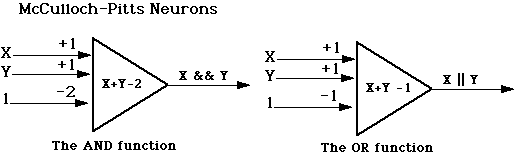
\includegraphics[width=6cm]{mpneuron.png}
	\caption{The McCollough-Pitts Neuron\cite{luger_2009}}
\end{figure}
\par
In 1958, the precursor of the modern-day neural network was born with Rosenblatt's development of the "perceptron."
Expanding on the MuCollough-Pitts representation of a neuron, his perceptron was a unit that similarly took in a set of inputs and calculated a weighted sum, activating with the sign function.  
\[ 
	sgn(\mathbf{x}) = \begin{cases}
		-1,& \big(\sum\limits_{i}w_ix_i\big) + b < 0\\
		+1,  &\text{Otherwise}
		\end{cases}
\]
\captionof{figure}{The Sign Function}
The key insight of Rosenblatt was that opposed to weights being fixed, they were adjustable parameters with positive and negative weights, and could 
hence be learned, however, his perceptron algorithm\cite{rosenblatt} was eventually criticized for being capable of charactering solely
linearly-separable decision boundaries and was most infamously incapable of computing the exclusive-or function.
\begin{figure}[H]
	\centering
	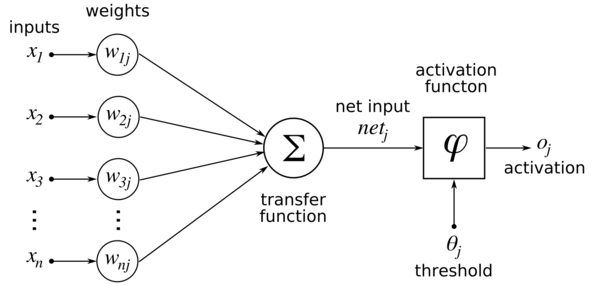
\includegraphics[width=6cm]{Rosenblattperceptron.png}
	\caption{The Rosenblatt Perceptron\cite{mitchell_1997}}
\end{figure}
The full history of perceptrons is outside the scope of this report, but after a period of falling out of fashion, the perceptron has made a massive resurgence in recent years due to the development of the ANN, where several perceptrons are combined in parallel and/or in layers to compute complex 
predictive models that can be applied to non-linearly separable decision boundaries. While the ANN was first developed in the 1960s, notably 
ADALINE and MADELINE\cite{widrow_hoff_1960}, it was not until the recent increases in both computational power and available data that their 
widespread use was adopted. Since then, these networks have had success in a vast collection of problems, ranging from natural language processing 
with recurrent neural networks, to computer vision with convolutional neural networks (CNNs).  
\par
A convolutional neural network is a popular tool used mainly in image classification and computer vision, but has been applied in recent years to a 
growing number of use cases. The basis of the CNN, and what makes it well suited to computer vision, is the convolutional layers. A convolution in this 
sense is a kernel with trainable weights which has the same depth of the image being convolved (i.e. and RGB image would have a depth of 3). However, 
the other dimensions of this kernel, or "filter," are usually smaller than on the other axes, which allows it to stride across windows of the image. The output 
of a single stride is a scalar, the sum of the element-wise product of the kernel with the input image. Each of these scalars is placed in a new grid, where
spacial relativity of the original image and the kernel outputs are preserved. By using several filters and layers of convolutions (and a lot of training data),
individual kernels can begin to recognize features such as edges and foreground, which when combined can lead to meaningful pattern recognition of the 
images.
\begin{figure}[H]
	\centering
	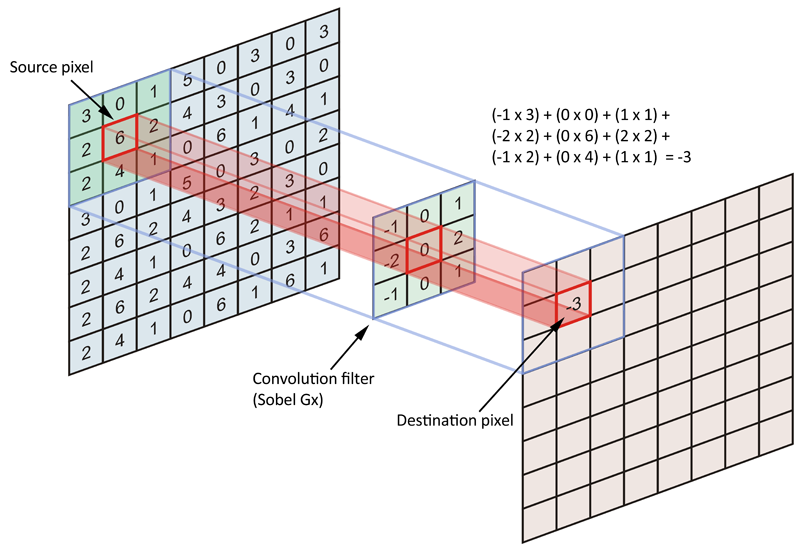
\includegraphics[width=6cm]{convolution.png}
	\caption{A convolution \cite{pjreddie}}
\end{figure}
\subsubsection{Deep Q-Learning}
\par
One of the methods we attempted to deploy to create an intelligent agent for Proximity was Deep Q-Learning, which combines the aforementioned 
techniques of Q-Learning and CNNs.  The motivation for this the parallel of the game board to an RGB image. It has three "depths," one each for a 
player's captured territory, and a discrete set of "pixel intensities," the value of the given territory, or -1 if the territory is claimed by an opponent, where 
the unclaimed channel's intensity is an indicator $\in \{-1,+1\}$ based upon whether or not it has been played.  The idea was to train a network to glean 
generalize Q-values based on a convolution of the game state, in addition to the current score, the current value of the tile to play, and the remaining move values of each player (in the discrete move value version of the game).
\par
Serving as a additional motivators were the results of Mnih, et al. in their paper "Human-level control through deep reinforcement learning"\cite{mnih}. In this paper, they were able to train agents through Deep Q-Learning through the following algorithm, which we imitated.
\begin{figure}[H]
	\centering
	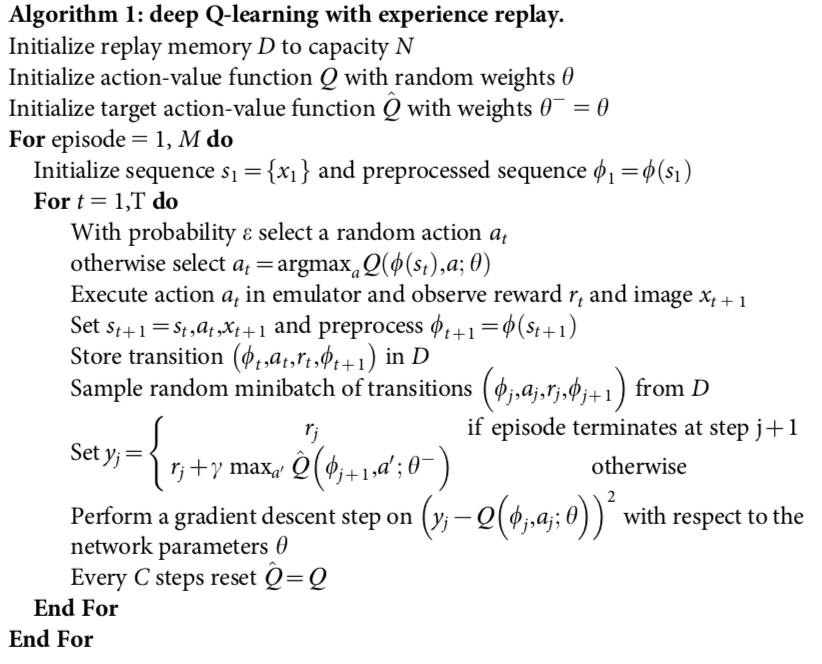
\includegraphics[width=8cm]{deepqalgo.png}
	\caption{Deep Q-Learning}
\end{figure}
\subsection{Project Description}
\par
Using the Keras %cite
deep learning library in Python with its functional API made it incredibly easy to build an ANN. Below is the network architecture.
\begin{figure}[H]
	\centering 
	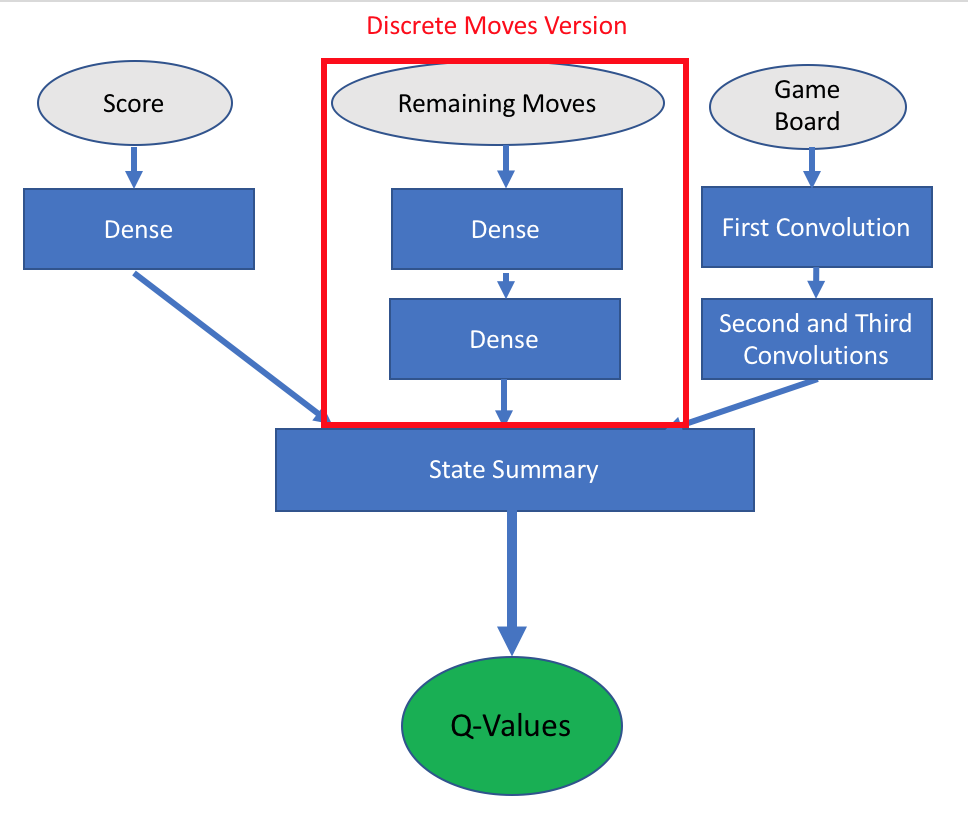
\includegraphics[width=8cm]{modelarch.png} 
	\caption{Model Architecture}
\end{figure}
\par
We used the rectified linear unit (ReLU) for the hidden layer activations, and merged the layers as a linear combination for the output layer.
 \begin{align}
	ReLU(x) &= \max(0, x) 
\end{align}
\captionof{figure}{The ReLU function}
Below are the relevant parameters of the networks: 
\subsubsection{Parameters}
\begin{itemize}
	\item
	Optimizer : Adam \cite{adam}
	\begin{itemize}
		\item
		Learning Rate : 0.001
		\item
		$\boldsymbol\beta_1$ : $0.9$
		\item
		$\boldsymbol\beta_2$ : $0.999$
	\end{itemize}
	\item
	Loss : Mean Squared Error
	\item
	Normalization : Batch Normalization on the Input Layer
	\item
	Dropout : Rate of 0.5 on all Hidden, Non-Convolutional Layers
	\item
	Batch Size : Range $[32, 512]$
	\item
	Epochs : Range $[10, 1000]$
	\item
	All other parameters can be found in \emph{qnetwork.py}
\end{itemize}
\subsubsection{Algorithm}
We used sample code to help implement the agent, making adjustments to suit the task at hand\cite{keon}. Her is the training pseudocode.
\begin{algorithmic}[1]
\Procedure{Train Q-Learning}{terminalReward}
\State wins $\gets 0$
\For{each experiment}
\State learner $\gets$ DeepQAgent(previousWeights)
\For{each episode}
\State reward wins $\gets 0$
\State game $\gets$ Proximity
\While{True}
\State val $\gets$ next value
\State state $\gets$ State(game, learner, val)
\State action $\gets$  learnerAction(game, state)
\State makeLearnerMove
\State makeOpponentMove
\State reward $\gets$ learnerScore - opponentScore
\If{gameOver}
\If{\small learnerScore $>$ opponentScore}\normalsize
\State reward $\gets$ terminalScore
\ElsIf{\small learnerScore $>$ opponentScore}
\State \normalsize reward $\gets$ terminalScore
\EndIf
\State nextState $\gets$ State(game, learner, val)
\State memoryReplay\\(state, action, reward, nextState, Terminal)
\State break
\EndIf
\State val $\gets$ next value
\State nextState $\gets$ State(game, learner, val)
\State memoryReplay\\(state, action, reward, nextState, NonTerminal)
\EndWhile
\EndFor
\State save trained weights
\EndFor
\EndProcedure
\end{algorithmic}
\section{Results}
Unfortunately, we ran into some major roadblocks in our first foray into Deep Reinforcement Learning. These included, but were not limited to:
\begin{itemize}
\item
\end{itemize}
\printbibliography
\end{document}